%%%%%%%%%%%%%%%%%%%%%%%%%%%%%%%%%%%%%%%%%%%%%%%%%%%%%%%%%%%%
\subsection{Estimated background rate in NEXT-100} \label{sec:BkgRate}
%%%
The contribution of each detector subsystem to the overall background rate of NEXT-100 is shown in Table~\ref{tab:BackgroundContributions}. These rates are obtained dividing the initial activities of \Tl\ and \Bi\ by the corresponding background rejection factors (defined as the inverse of the background acceptance resulting from the \bbonu-decay event selection described in the previous section). They are also represented graphically in Figure~\ref{fig:BackgroundContributions}. The photosensors are, by far, the dominant source of background in NEXT-100. Notice, however, that our knowledge is, in any case, quite uncertain, given that for most background sources we only have at present a limit to their activity. This is, in fact, a problem common to all \bbonu-decay experiments, and it will be even more serious for the experiments of the tonne scale, which will require materials and components of higher radiopurity.


%%%%%%%%%%
\begin{sidewaystable}
\centering
\caption{Contribution to the background rate of NEXT-100 predicted for each subsystem of the detector considered in our background model. The second and third columns correspond to the initial activities of \Tl\ and \Bi\ (see Table~\ref{tab:RadioactivityBudget}). The fourth and fifth columns contain the rejection factors computed with the detector simulation. The last two columns in the table show the background rate estimated for each subsystem (i.e.\ the ratio of the previous quantities) expressed in $10^{-4}$~\ckky. For most subsystems, we only have upper limits to their induced background rate. In those cases where we have a positive measurement, the figures in parentheses give the 1-sigma uncertainty in the last digit.} \label{tab:BackgroundContributions}
%%%
\small
\begin{tabular*}{.9\textheight}{@{\extracolsep{\fill}} l *{2}{c} *{2}{l} *{2}{D{.}{.}{4.4}}}
\toprule
%%%
Detector subsystem & \multicolumn{2}{c}{Activity (mBq)} & \multicolumn{2}{c}{Rejection factor} & \multicolumn{2}{c}{$c$ $\left(\mathrm{10^{-4}/(keV~kg~yr)}\right)$} \\ \cmidrule(lr){2-3} \cmidrule(lr){4-5} \cmidrule(l){6-7}
       & \multicolumn{1}{c}{\Tl} & \multicolumn{1}{c}{\Bi} & \multicolumn{1}{c}{\Tl} & \multicolumn{1}{c}{\Bi} & \multicolumn{1}{c}{\Tl} & \multicolumn{1}{c}{\Bi} \\ \midrule
%%%
\emph{Pressure vessel} \\
%
\quad Total & $<197$ & $<603$ & $1.0(3)\times10^{8}$ & $1.0(5)\times10^{9}$ & <0.23 & <0.07 \\ \addlinespace
%%%
\emph{Energy plane} \\
%
\quad PMTs & $12(3)$ & $<56$ & $4.1(3)\times10^{6}$ & $6.1(5)\times10^{6}$ & 0.35(9) & <1.1 \\
%
\quad PMT enclosures & $<0.34$ & $<2.6$ & $6.8(6)\times10^{6}$ & $9.5(9)\times10^{6}$ & <0.006 & <0.04 \\
%
\quad Enclosure windows & $0.34(8)$ & $<2.6$ & $2.38(11)\times10^{6}$ & $2.56(13)\times10^{6}$ & 0.017(4) & <0.12 \\
%
\quad Support plate & $<0.6$ & $<5$ & $5.0(4)\times10^{6}$ & $1.43(16)\times10^{7}$ & <0.014 & <0.04 \\ \addlinespace
%%%
\emph{Tracking plane} \\
\quad SiPMs & $<5$ & $<18$ & $2.04(8)\times10^{6}$ & $2.04(8)\times10^{6}$ & <0.29 & <1.1 \\
\quad SiPM boards & $1.5(2)$ & $3.2(1.1)$ & $2.04(8)\times10^{6}$ & $2.04(8)\times10^{6}$ & 0.088(13) & 0.19(6) \\ \addlinespace
%%%
\emph{Electric-field cage} \\
\quad Barrel & $<1$ & $<8$ & $2.61(13)\times10^{6}$ & $2.27(10)\times10^{6}$ & <0.05 & <0.4 \\ 
\quad Shaping rings & $<0.5$ & $<4$ & $2.61(13)\times10^{6}$ & $2.27(10)\times10^{6}$ & <0.023 & <0.23 \\
%
\quad Electrode rings & $<1.5$ & $<5$ & $2.61(13)\times10^{6}$ & $2.27(10)\times10^{6}$ & <0.07 & < 0.24 \\
%
\quad Anode plate & $0.092(17)$ & $0.7(3)$ & $2.04(8)\times10^{6}$ & $2.04(8)\times10^{6}$ & 0.005(1) & 0.039(17) \\
%
\quad Resistor chain & $<0.0026$ & $<0.0013$ & $2.61(13)\times10^{6}$ & $2.27(10)\times10^{6}$ & <0.00012 & <0.0011 \\ \addlinespace
%%%
\emph{Shielding} \\
\quad Inner shield & $<13$ & $<111$ & $9.3(9)\times10^{6}$ & $1.9(3)\times10^{7}$ & <0.17 & <0.7 \\
\quad Outer shield & $2060(430)$ & $21300(4300)$ & $1.0(5)\times10^{10}$ & $1.0(5)\times10^{10}$ & 0.025(13) & 0.25(14) \\
\bottomrule
\end{tabular*}
\end{sidewaystable}
%%%%%%%%%%


%%%%%%%%%%
\begin{figure}
\centering
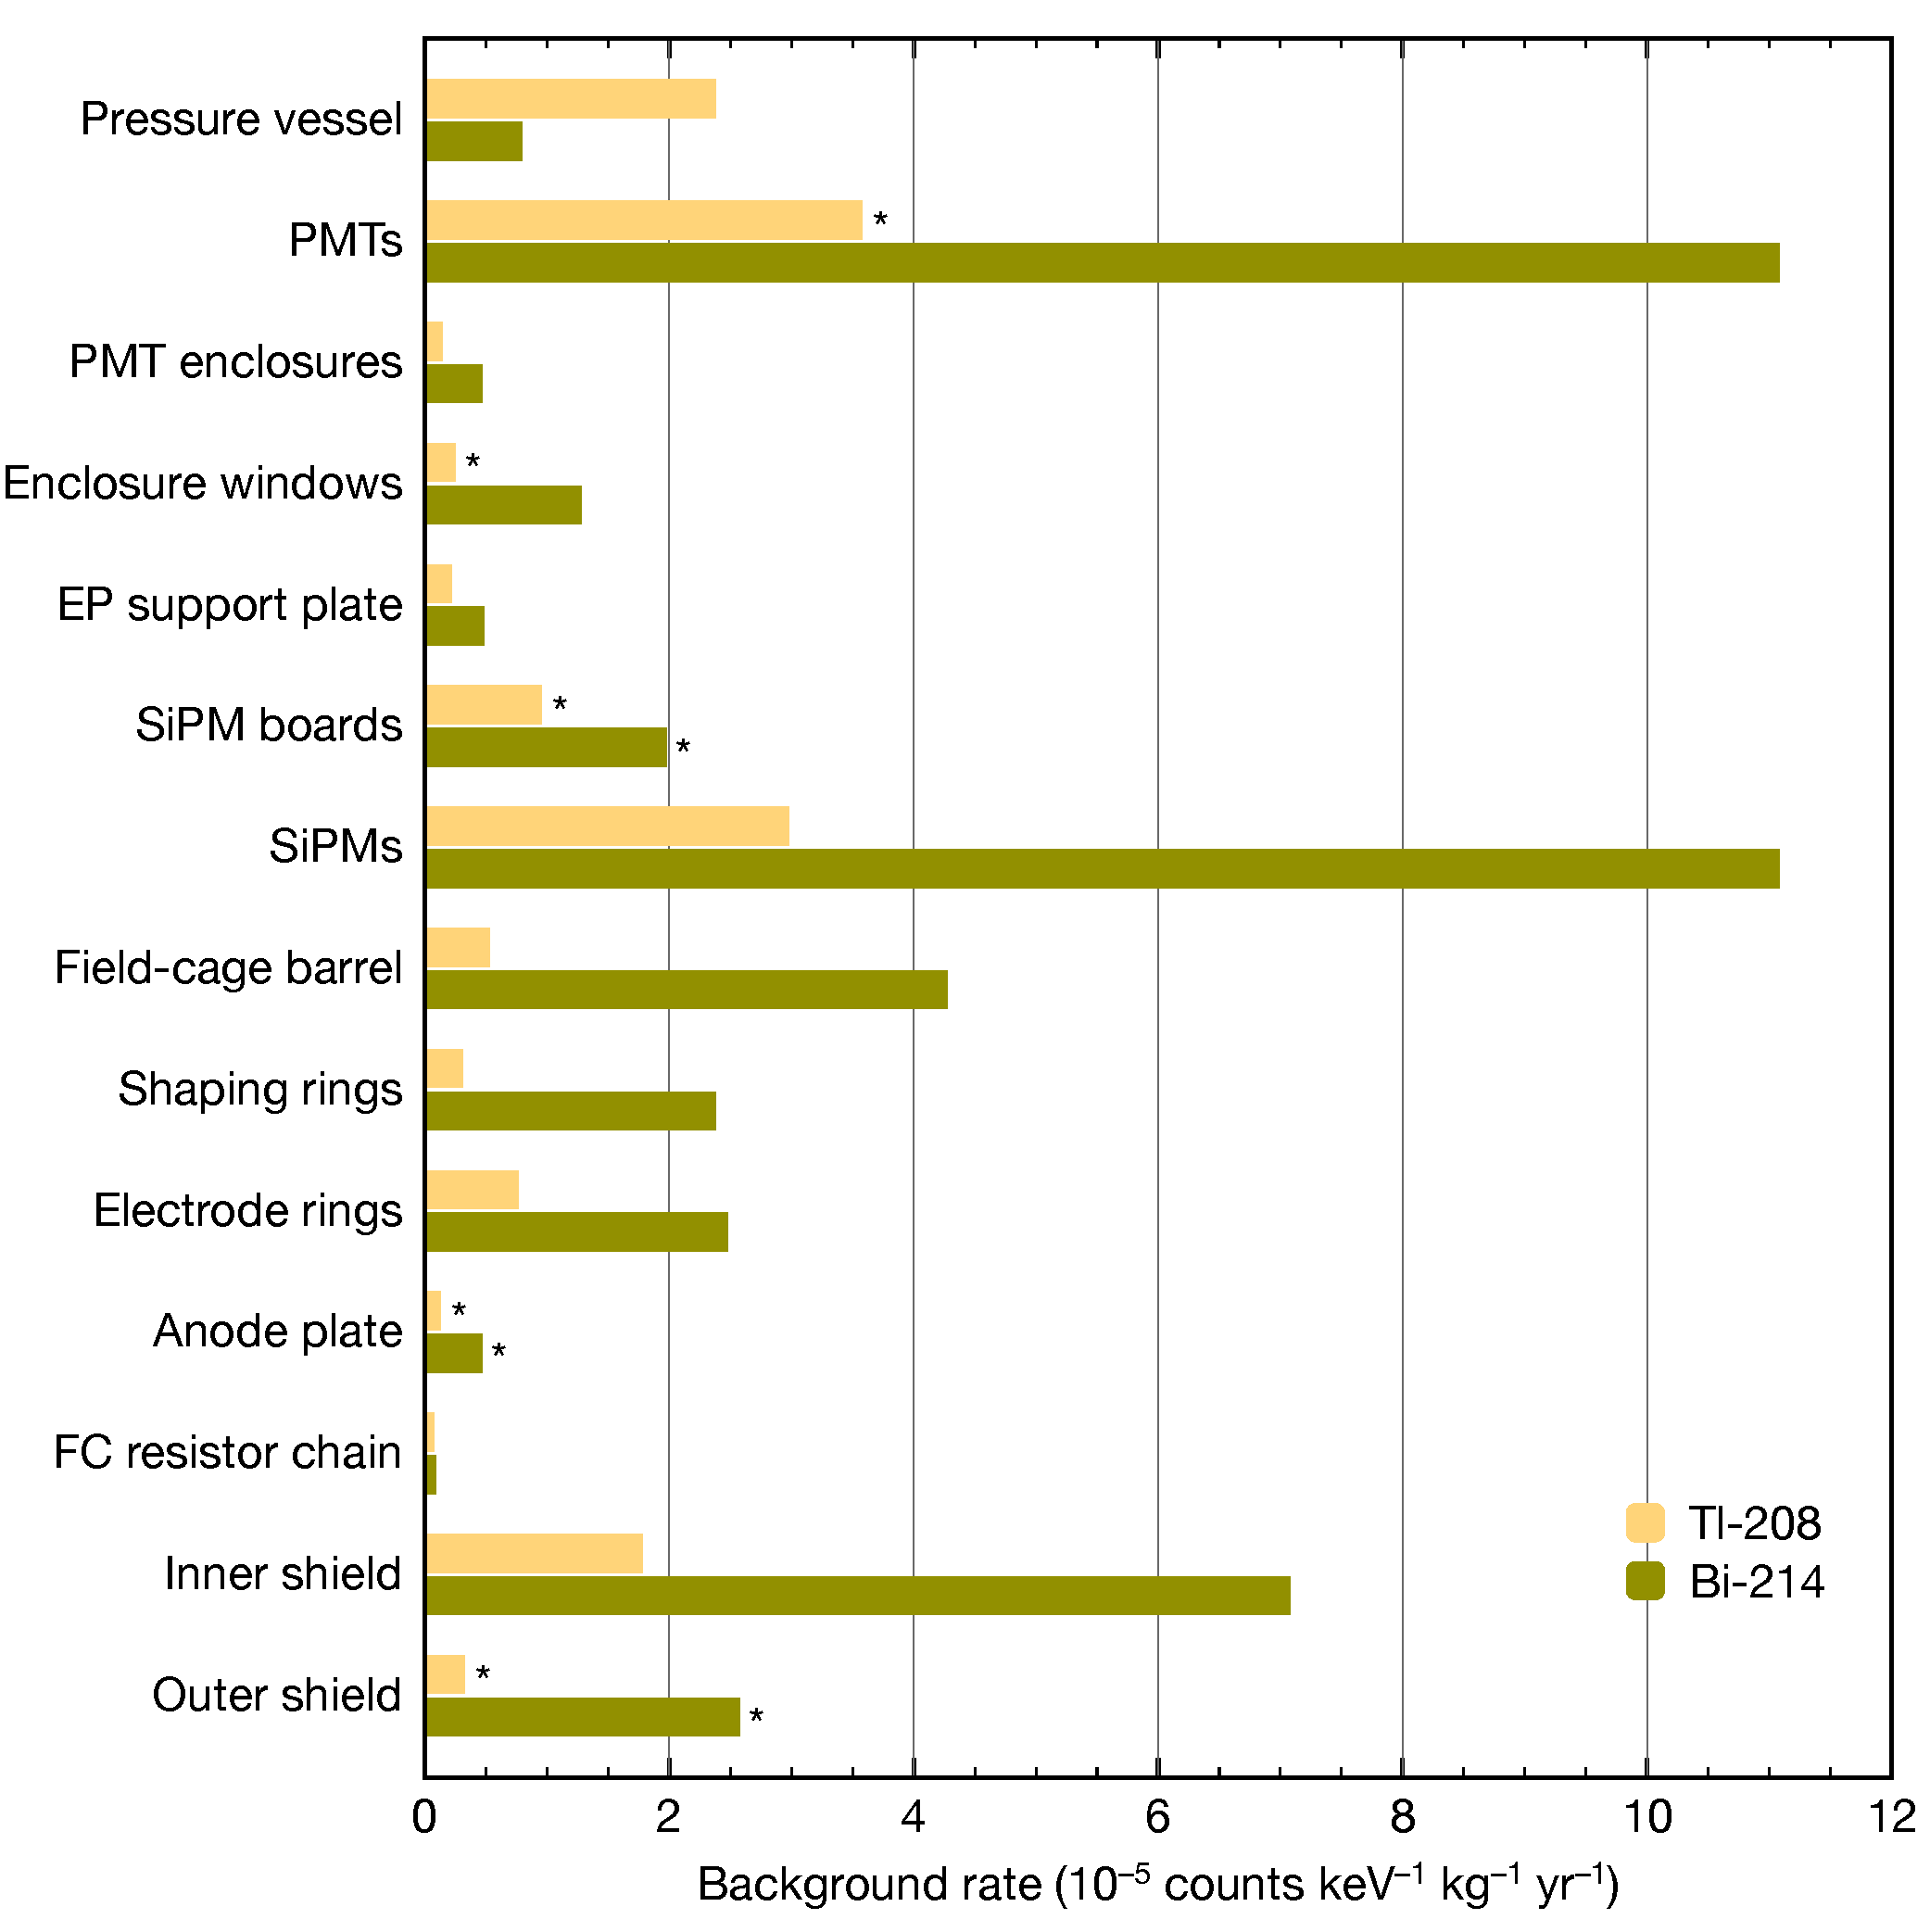
\includegraphics[width=0.9\textwidth]{img2/BackgroundSources.pdf}
\caption{Contribution to the background rate of NEXT-100 of the different detector subsystems considered in our background model. An asterisk (*) next to a bar indicates that the contribution corresponds to a positive measurement of the activity of the material.} \label{fig:BackgroundContributions}
\end{figure}
%%%%%%%%%%

%%%%%%%%%%
\begin{table}
\centering
\caption{Contribution of major subsystems to the expected background rate of NEXT-100, expressed in 10$^{-4}$ counts~keV$^{-1}$~kg$^{-1}$~yr$^{-1}$.} \label{tab:BkgRateSummary}
\begin{tabular*}{.8\textwidth}{@{\extracolsep{\fill}} l *{3}{D{.}{.}{4.6}}}
\toprule
Detector subsystem & \multicolumn{1}{c}{\Tl} & \multicolumn{1}{c}{\Bi} & \multicolumn{1}{c}{\itshape Total} \\ \midrule
Pressure vessel     & <0.23 & <0.07 & <0.31 \\
Energy plane        & <0.38 & <1.31 & <1.69 \\
Tracking plane      & <0.38 & <1.27 & <1.65 \\
Electric-field cage & <0.14 & <0.93 & <1.07 \\
Inner shield        & <0.17 & <0.70 & <0.87 \\
Outer shield        & 0.025(13) & 0.25(14) & 0.28(14) \\
{\itshape Total}    & <1.33 & <4.53 & <5.86 \\ 
\bottomrule
\end{tabular*}
\end{table}
%%%%%%%%%%

%%%%%%%%%%
\begin{figure}
\centering
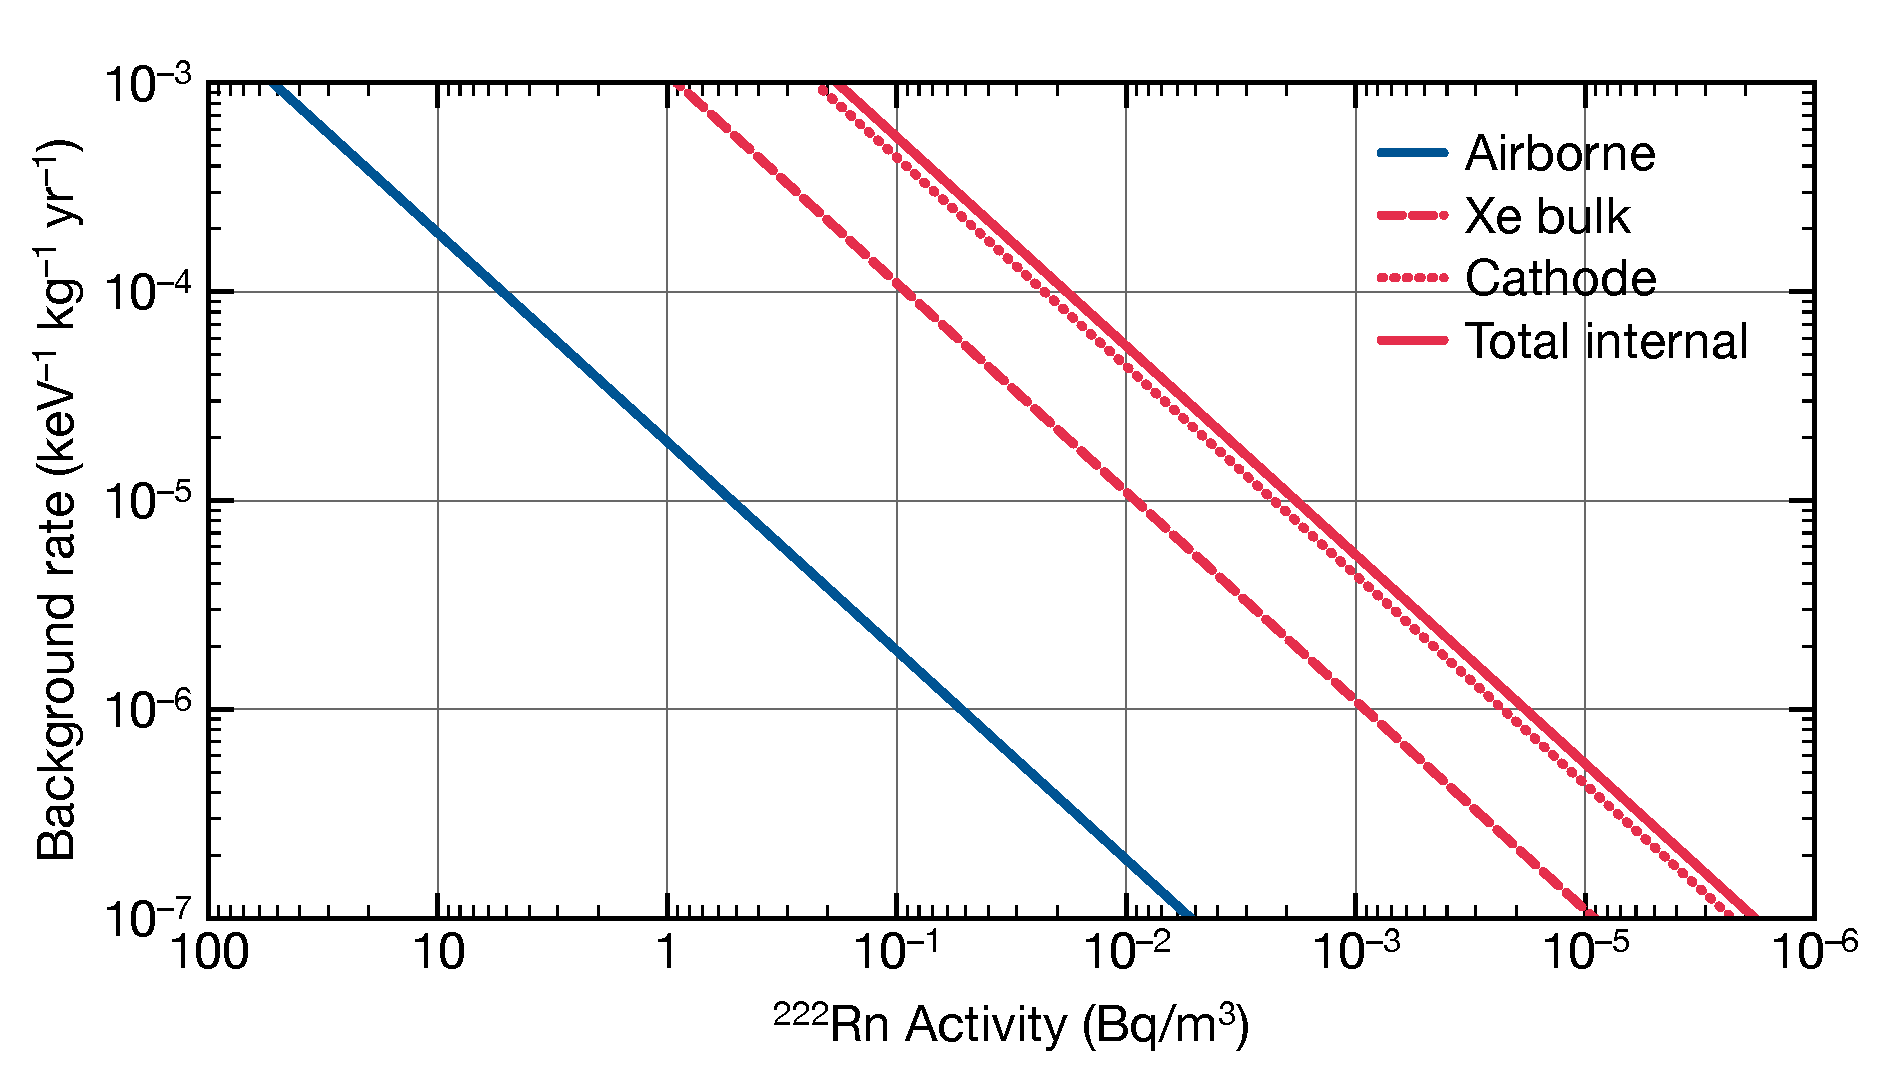
\includegraphics[width=0.9\textwidth]{img2/RadonNext100.pdf}
\caption{Background rate induced in NEXT-100 by airborne radon and radon contamination in the xenon gas (labelled as \emph{internal}) in terms of the activity of $^{222}$Rn.} \label{fig:RadonNext100}
\end{figure}
%%%%%%%%%%


Table~\ref{tab:BkgRateSummary} shows the contributions grouped into six major subsystems. The background from \Bi\ is 4.3 times more abundant than the background from \Tl. The overall background rate estimated for NEXT-100 is
%%%
\begin{equation}
<5.86\times10^{-4}~\mathrm{counts/(keV~kg~year)}\,.
\end{equation}
%%%
This rate includes only radioactive backgrounds from detector materials and components. All other sources of background are expected to contribute at the level of $10^{-5}$~keV$^{-1}$~kg$^{-1}$~yr$^{-1}$ or below:
%%%
\begin{itemize}
\item The activity of airborne radon in the vicinity of the detector --- which translates, ultimately, into \Bi\ activity on the internal surface of the lead shield and on the external surface of the vessel--- will be reduced  by at least two orders of magnitude with respect to the activity in the experimental hall of LSC ($\sim$80~Bq/m$^{3}$) thanks to the use of a radon mitigation machine or the removal of the air inside the lead shield (3.2~m$^{3}$) with clean nitrogen. The computed rejection factor for this source of background is $2\times10^{9}$, resulting in a background rate of about $10^{-5}$~keV$^{-1}$~kg$^{-1}$~yr$^{-1}$ for a $^{222}$Rn activity of 0.5~Bq/m$^{3}$ (see Figure~\ref{fig:RadonNext100} for other values of the specific activity of $^{222}$Rn in the range between 10$^{-2}$ and 10$^{2}$~Bq/m$^{3}$).
%
\item Radon contamination in the xenon gas causes two different types of background events: $\beta$ tracks from the decay of \Bi\ in the active volume, and photoelectrons generated by gamma rays emitted, for the most part, from the TPC cathode following the decay of \Bi. In the EXO-200 TPC, the latter type of events constitute about 80\% of the measured activity of $^{222}$Rn in the liquid xenon, while the former make up the remaining 20\% \cite{Albert:2013gpz}. The rejection power against both types of background events is similar, approximately $2.5\times10^{6}$. In the case of the $\beta$ decays of \Bi\ in the xenon bulk, we have assumed that Bi-Po tagging --- i.e.\ the coincident detection in an event of the $\beta$ emitted in the decay of \Bi\ and the alpha emitted by $^{214}$Po shortly after--- can be done with high efficiency ($\gtrsim99\%$). Figure~\ref{fig:RadonNext100} (red lines) shows the background rate generated in NEXT-100 by this internal contamination of radon in terms of the activity of $^{222}$Rn. In order for this background to contribute, at most, at the level of $10^{-5}$~keV$^{-1}$~kg$^{-1}$~yr$^{-1}$, radon activities in the xenon gas below a few mBq per cubic metre will be required. The EXO-200 detector, which has been operating without a radon suppression system, has measured, for instance, an activity of $^{222}$Rn of that order in their xenon volume: $(3.65\pm0.37)~\mu\mathrm{Bq/kg}$ \cite{Albert:2013gpz}. Similarly, the radon activity of the NEMO-3 tracking gas was measured to be about 5~mBq/m$^{3}$ \cite{Arnold:2013dha}.
%
\item Out of the 50 atoms of $^{137}$Xe produced on average every year by neutron activation of \Xe\ (\textsection~\ref{subsec:MuonsNeutrons}), 0.25 of them will decay emitting a $\beta$ track with energy within our region of interest. These events will be suppressed by about a factor of 10 by the 2-blobs selection criterion, yielding a background rate of approximately $9\times10^{-6}$~keV$^{-1}$~kg$^{-1}$~yr$^{-1}$. Nevertheless, the neutron flux can be attenuated by several orders of magnitude using polyethylene shielding of a few tens of centimetres in thickness.
\end{itemize}
%%%







